\section{Introduction and Open Loop
Discussion}\label{introduction-and-open-loop-discussion}

\begin{wrapfigure}{r}{0.62\textwidth}
  \begin{center}
  \vspace{-20pt}
  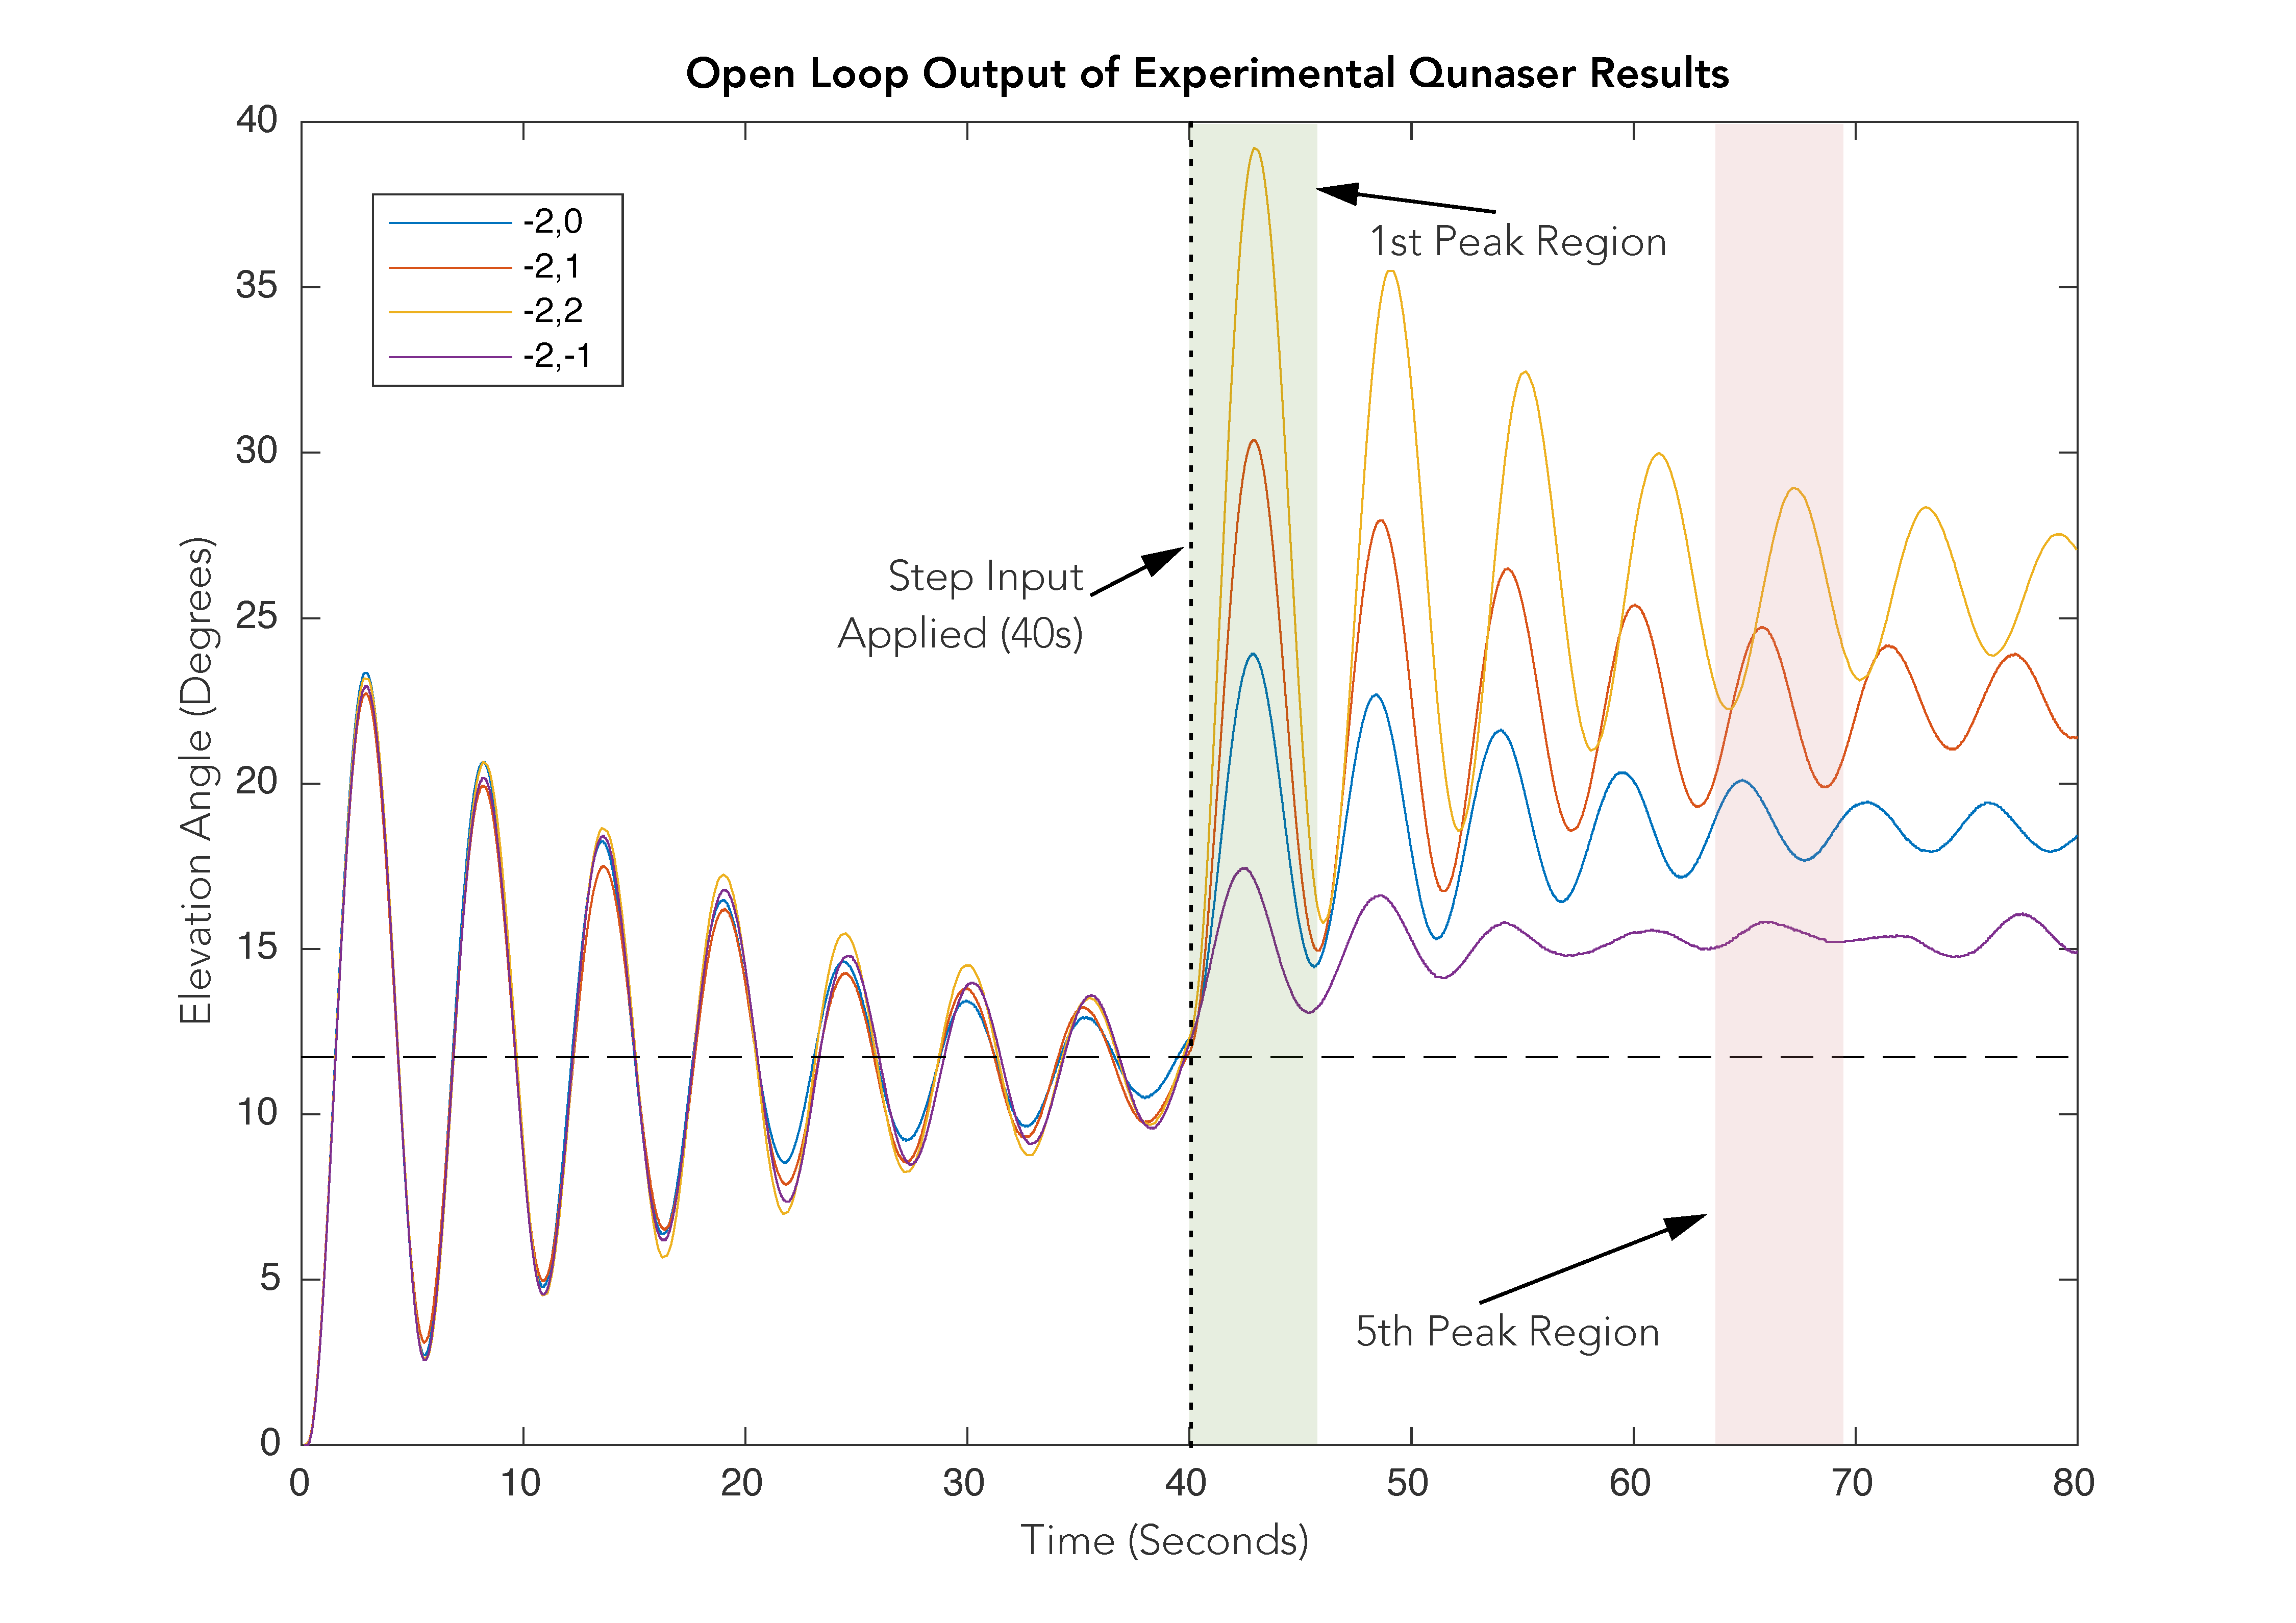
\includegraphics[trim = 150 60 180 20, clip, width=0.615\textwidth]{intrograph.pdf}
  \end{center}
  \caption{Graph Showing the Open Loop Nature of the Experimental Quanser Response}
  \label{intrograph}
  \vspace{-15pt}
\end{wrapfigure}

This report compares the experimental and analytical transfer functions
of a 3-degrees-of-freedom Quanser-Control rig. Control system design is
important in understanding the behaviour of dynamic systems, to improve
the performance. Sensors and actuators are used in the Quanser to
measure and vary performance characteristics of the Quanser. In this
experiment, an elevation angle change was introduced to the Quanser
revealing an oscillating damped behaviour. Measuring this response an
empirical transfer function was then created, to closely match the
observed behaviour.

An Open-Loop system is a where behavioural characteristics can be
controlled manually. These changes are not fed back into the system,
therefore the output has no effect on the input of the system
\cite{openloop}; meaning self-correction is not possible. In the case of
the Quanser-Control Rig, elevation angle was independent of the output
and was manually controlled, whereas pitch and travel data was manually
fed back to the system. Figure \ref{intrograph} shows the open loop
behaviour of the elevation axis, as the elevation angle was varied
between 10 and 40 degrees.

\section{Method}\label{method}

\subsection{Finding Experimentation Results from
Quansers}\label{finding-experimentation-results-from-quansers}

\begin{enumerate}

\item
  Replace the elevator input with a step block, using the parameters:
  Start Time: 40s, Start Value: -2, End Value: -1 to 2. This was used to
  automate the step input at a specific time for each elevator input
  test. A step input time of 40s was chosen to allow the initial
  response to settle to an acceptable level (see Figure
  \ref{intrograph}).
\item
  Use range of elevator input values, varying from an initial value of
  -2 to 2 in steps of 1. Repeat each test case, saving workspace
  variables.
\item
  Check the data for anomalies, average valid repeats to obtain the
  experimental response across the different step inputs, see Figure
  \ref{intrograph}.
\end{enumerate}

\subsection{Analyse Transfer Function}\label{analyse-transfer-function}

Isolate elevation values for corresponding inputs from 40s to 80s; this
captures the response after the step input.In order to estimate the
transfer function, the following parameters were calculated: Natural
Frequency \(\omega_d\), Undamped Natural Frequency \(\omega_n\) and the
Damping ratio \(\zeta\). Refer to Table \ref{eqtable} for equations
used.

\subsubsection{Second Order}\label{second-order}

To calculate the Second Order Transfer-Function, a forced response
behaviour was noted. Using Table \ref{eqtable} equations and the x and y
values taken from the peaks highlighted in Figure \ref{intrograph}, the
logarithmic decrement and the period of damped oscillation was
approximated. Using these equations values for the Damping Ratio
\(\zeta\) and Natural Frequency \(\omega_n\) were obtained and
substituted into the formal equation shown in equation \ref{2otf}.

\begin{wrapfigure}{r}{0.6\textwidth}
\vspace{-25pt}
  \centering
  \captionof{table}{Table Showing Key Parameter Calculations \cite{vibnote},\cite{vibnote2}}
  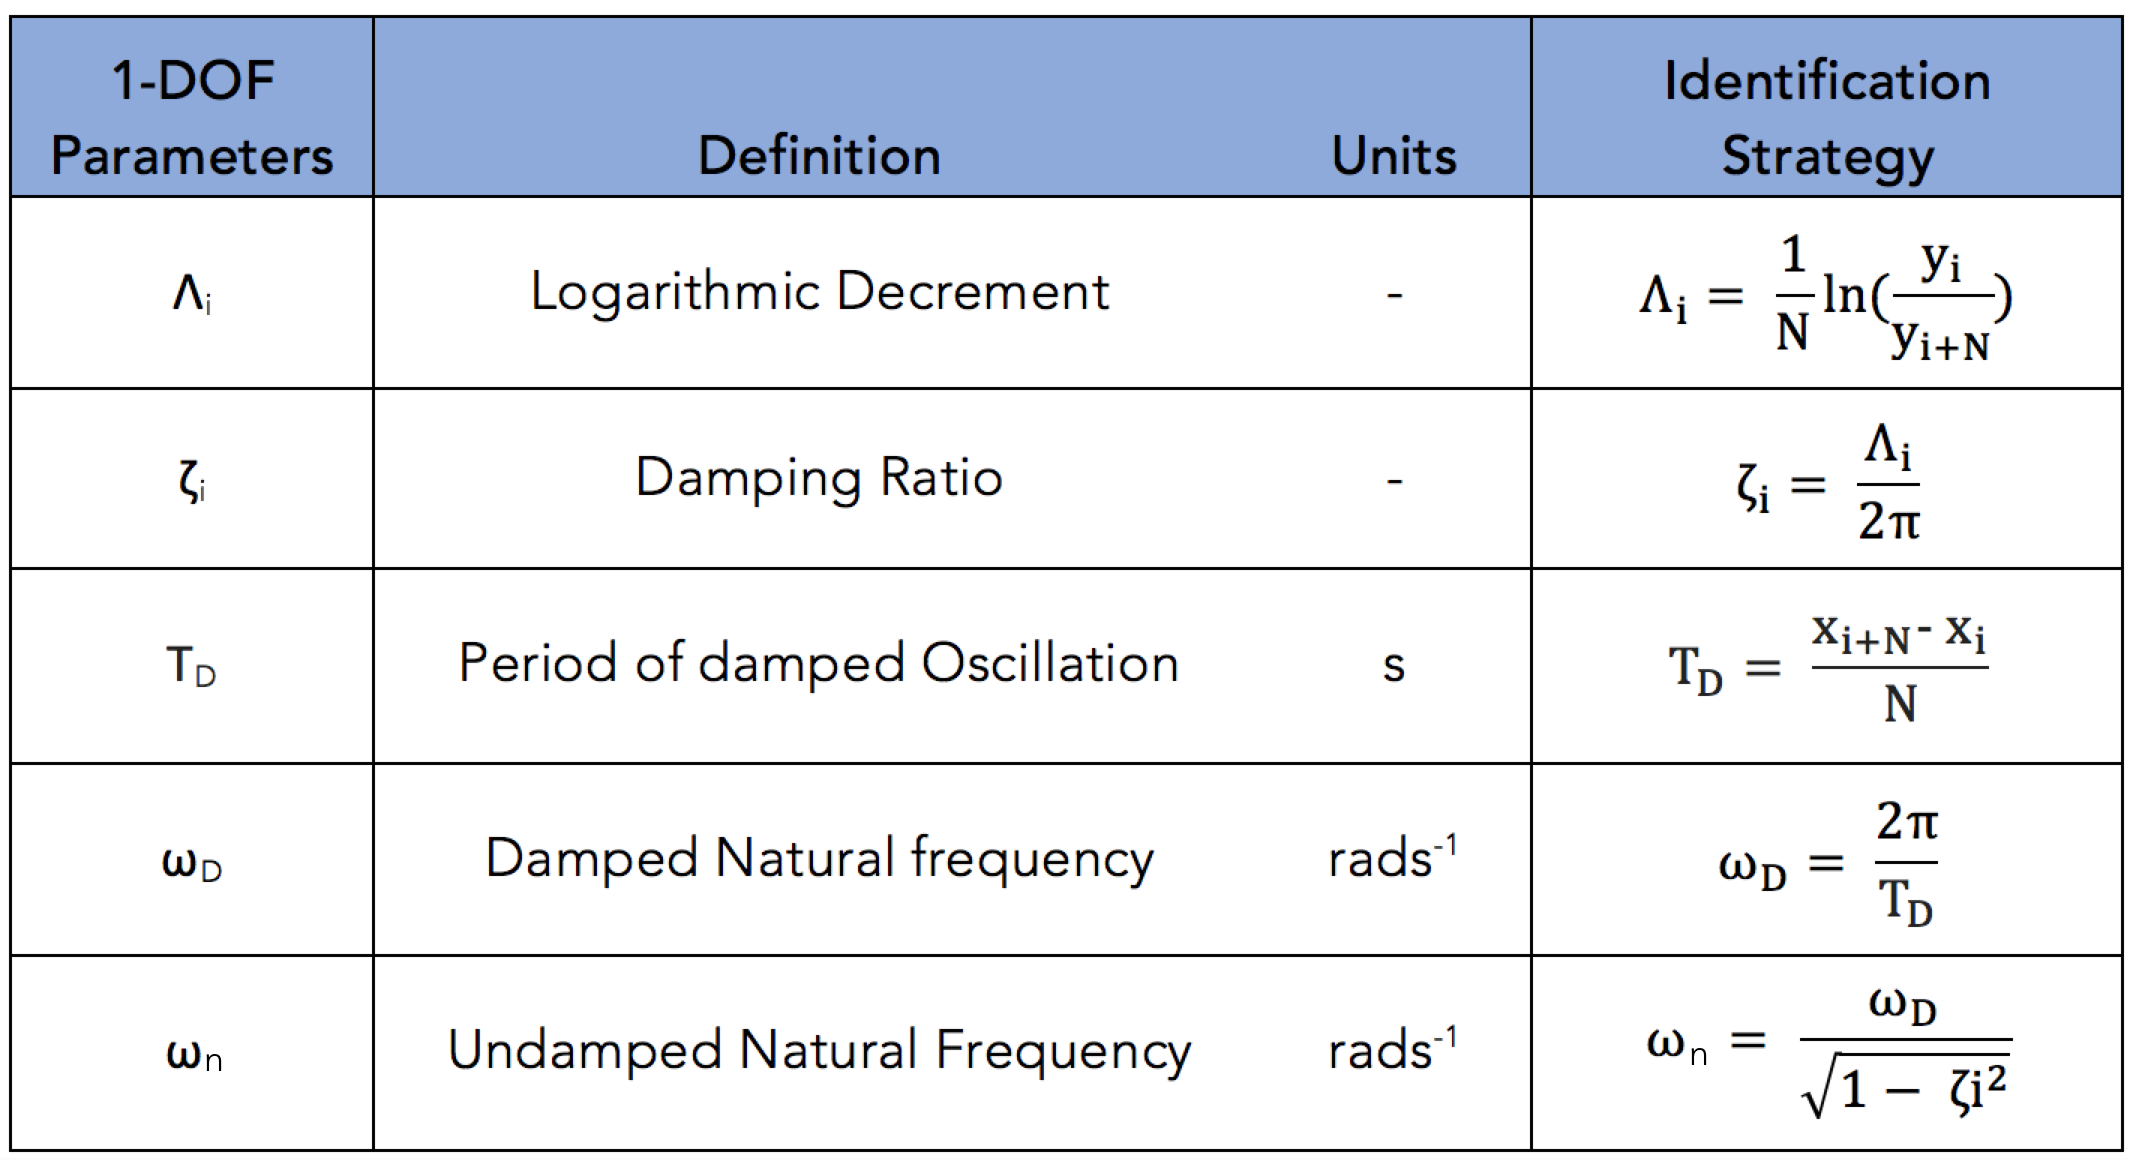
\includegraphics[trim = 0 0 0 0, clip, width=\linewidth]{eqtable.png}
  \label{eqtable}
\end{wrapfigure}

\begin{align}
\frac{ y(s) }{ u(s) } &=\frac{ k\cdot \omega_{ n }^{ 2 } }{ s^{ 2 }+2\zeta \omega_{ n }s+\omega_{ n }^{ 2 } } \label{2otf}
\end{align}

In order to obtain a single transfer function which represents the
system as a whole for varying elevators angle steps, analytical transfer
functions were found for each test case. These parameters were then
averaged obtaining a single fit transfer function where gain was changed
to model different elevator angle step inputs. This captured some of the
behaviour of the system as step level varied.

\begin{wrapfigure}{r}{0.5\textwidth}
  \begin{center}
\vspace{-25pt}
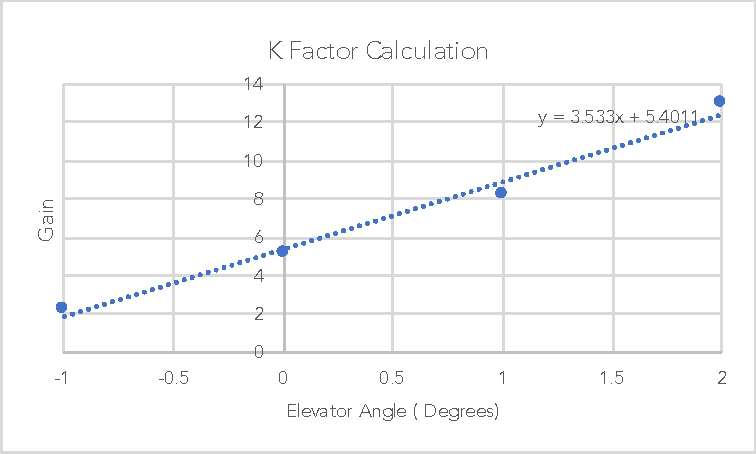
\includegraphics[trim = 10 10 10 10, clip, width=0.49\textwidth]{kgraph.pdf}  
\end{center}
\caption{Graph Finding the Gain For Each Step Input}
\label{kgraph}
  \vspace{-15pt}
\end{wrapfigure}

To calculate a representative gain scaling factor \(k\) for each of the
step inputs, max elevation for each step input was taken (from the first
peak shown in Figure \ref{intrograph}). These values were plotted to
find their correlation, shown in figure \ref{kgraph}. The gain \(k\)
value was heuristically adjusted to match the analytical amplitude with
the experimental results from -2 to 2, where \(k = 0.26\) showed a good
fit. This value was used to translate the correlation equation between
points into scaling factors.

After applying this method, amplitudes for all the steps fitted more
closely. Finally damping ratio and undamped natural frequency were
tweaked to give the final fit, again by trial and error.

\subsubsection{First Order}\label{first-order}

\begin{align}
 &\text{Standard First Order Response Transfer Function:} &&\frac { y(s) }{ u(s) } =\frac { k }{ \tau s+1 }
\label{fos}
\end{align}

Due to the Quanser-Control Rig being a Second Order System, Equation
\ref{fos} was not applicable for finding the First Order Transfer
Function. Instead this was estimated by considering the Second Order
Transfer Function case where: \(\zeta =1\) and \(s^2=0\).

\begin{align}
\frac { k\cdot \omega_{ n }^{ 2 } }{ s^2 + 2\zeta \omega_{ n }s+\omega_{ n }^{ 2 } } &\rightarrow \frac { k\cdot \omega_{ n }^{ 2 } }{ 2\omega_{ n }s+\omega_{ n }^{ 2 } }
\end{align}

\section{Results}\label{results}

\begin{align}
&\text{2nd Order Transfer Function}: && k \cdot \frac { 1.109 }{ s^{ 2 }+0.1313s+1.109 }
\end{align}

\begin{align*}
&\text{Where:} &&\zeta = 0.0623, \quad \omega_n = 1.0532
\end{align*}

\begin{align}
&\text{1st Order Transfer Function}: && k \cdot \frac { 1.109 }{ 2.106s+1.109 }
\end{align}

\begin{align*}
&\text{Where:} &&\zeta = 1 &&& \omega_n = 1.0532
\end{align*}

\begin{figure}[H]
\centering
\begin{minipage}{.49\textwidth}
\centering
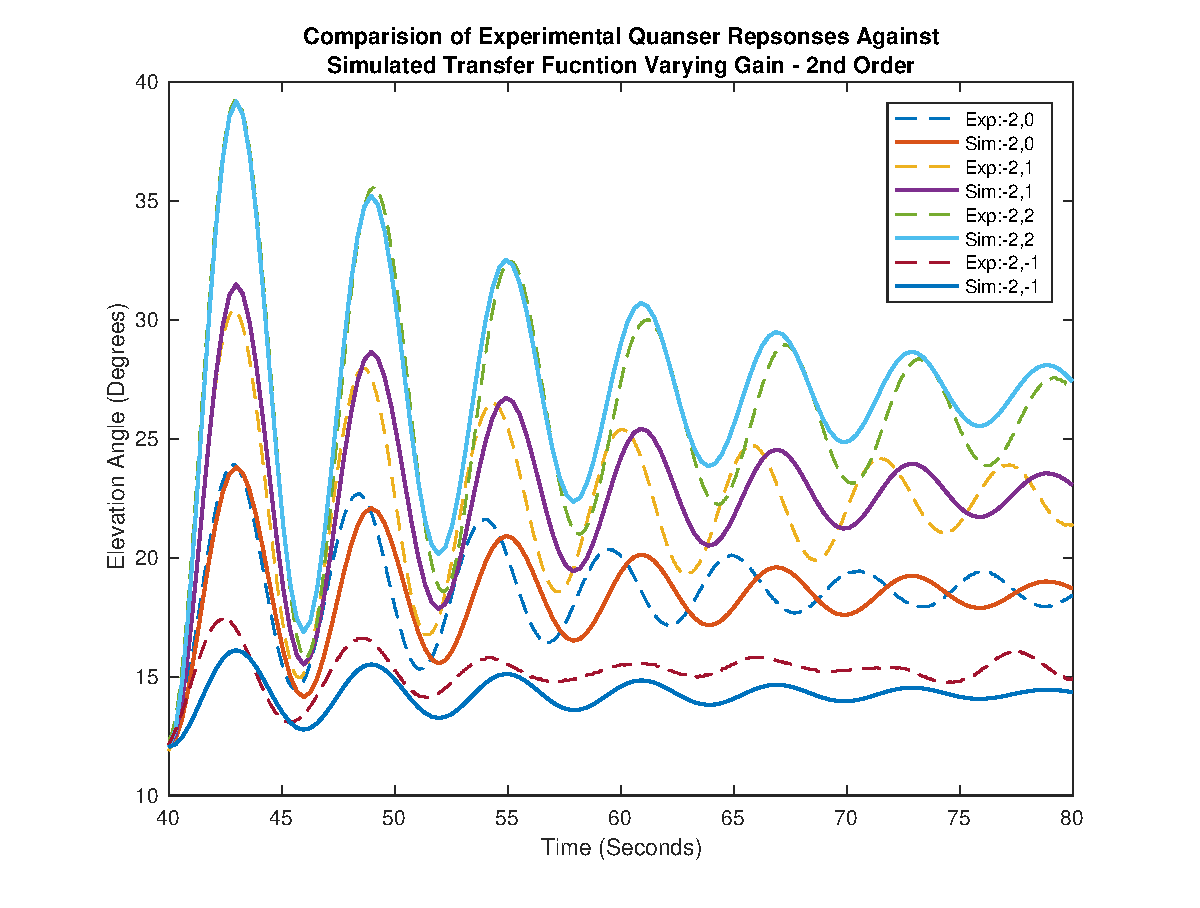
\includegraphics[trim = 35 16 35 0, clip, width=0.995\textwidth]{2ndTFcomp.eps}
\caption{2nd Order Simualted Transfer Function Comparision}
\label{2ndTFcomp}
\end{minipage}
\hfill
\begin{minipage}{.49\textwidth}
  \centering
  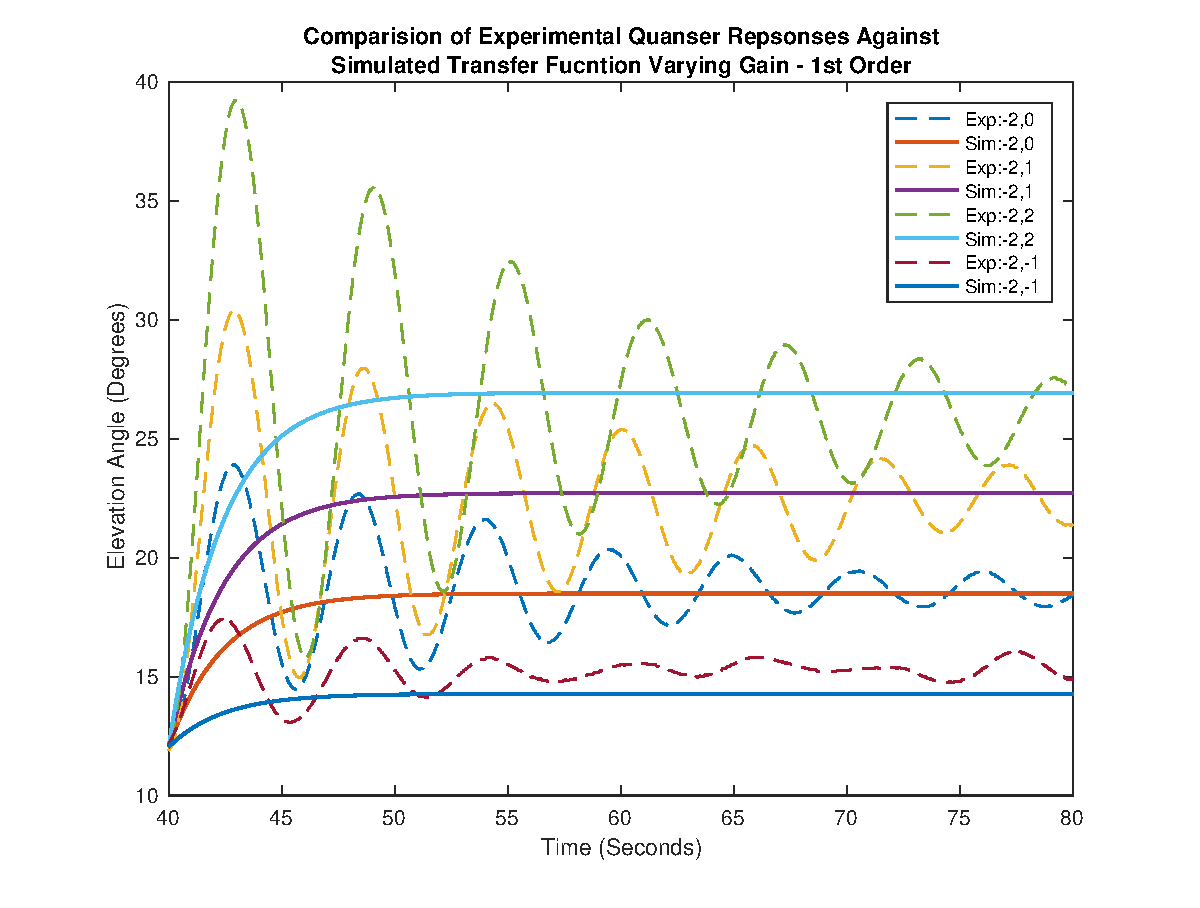
\includegraphics[trim = 35 16 35 0, clip, width=0.995\textwidth]{1stTFcomp.eps}
  \caption{1st Order Simualted Transfer Function Comparision}
  \label{1stTFcomp}
\end{minipage}
\vspace{-11pt}
\end{figure}

\begin{figure}[H]
\centering
\begin{minipage}{.49\textwidth}
Second Order Step Information:
\begin{align*}
t_r &= 1.0385 &&t_s = 57.3382
\end{align*}
\end{minipage}
\hfill
\begin{minipage}{.49\textwidth}
First Order Step Information:
\begin{align*}
t_r &= 4.1719 &&t_s = 7.4287
\end{align*}
\end{minipage}
\vspace{-11pt}
\end{figure}

\section{Observations and Analysis:}\label{observations-and-analysis}

\subsection{Experimental Elevator
Input:}\label{experimental-elevator-input}

\begin{itemize}
\tightlist
\item
  There is an observable phase and amplitude deviation, particularly
  after the third peak. The phase shift becomes increasingly out of
  phase as the initial step input is reduced.
\item
  Peak amplitude prediction becomes worse for lower amplitude cases,
  however there is a very good match for 0,1 and 2 test cases first
  three peaks, the k value equation provided a good match. Note this
  equation was set heuristically to a step input of 2.
\item
  The oscillations around the expected steady level were slightly larger
  above the steady state level rather than below. This could be an
  artefact of the Quanser accumulating elevation drift.
\item
  Steady state values match well for an elevator input of 0 and 1,
  however are noticeably different for -1 and 2.
\end{itemize}

\subsection{\texorpdfstring{Root-Locus plot (See Figure
\ref{poleszmap})}{Root-Locus plot (See Figure )}}\label{root-locus-plot-see-figure}

\begin{itemize}
\tightlist
\item
  The grid lines represent lines of constant damping and lines of
  natural frequency
\item
  The Second Order Transfer Function Root-Locus has a pair of points
  with an imaginary axis component (complex root) - This shows the
  stable underdamped nature of the system as \(0<\zeta<1\)
\item
  The First Order Transfer Function Root-Locus diagram point exists
  purely in the real axis component, meaning the function is critically
  damped as expected and stable.
\item
  Increase in gain for the Second Order shows the roots becoming more
  positive and negative in the imaginary axis respectively
\item
  Increase in gain for the First Order shows the root becoming more
  negative along the real axis
\end{itemize}

\section{Discussion}\label{discussion}

\begin{wrapfigure}{r}{0.56\textwidth}
  \begin{center}
  \vspace{-40pt}
  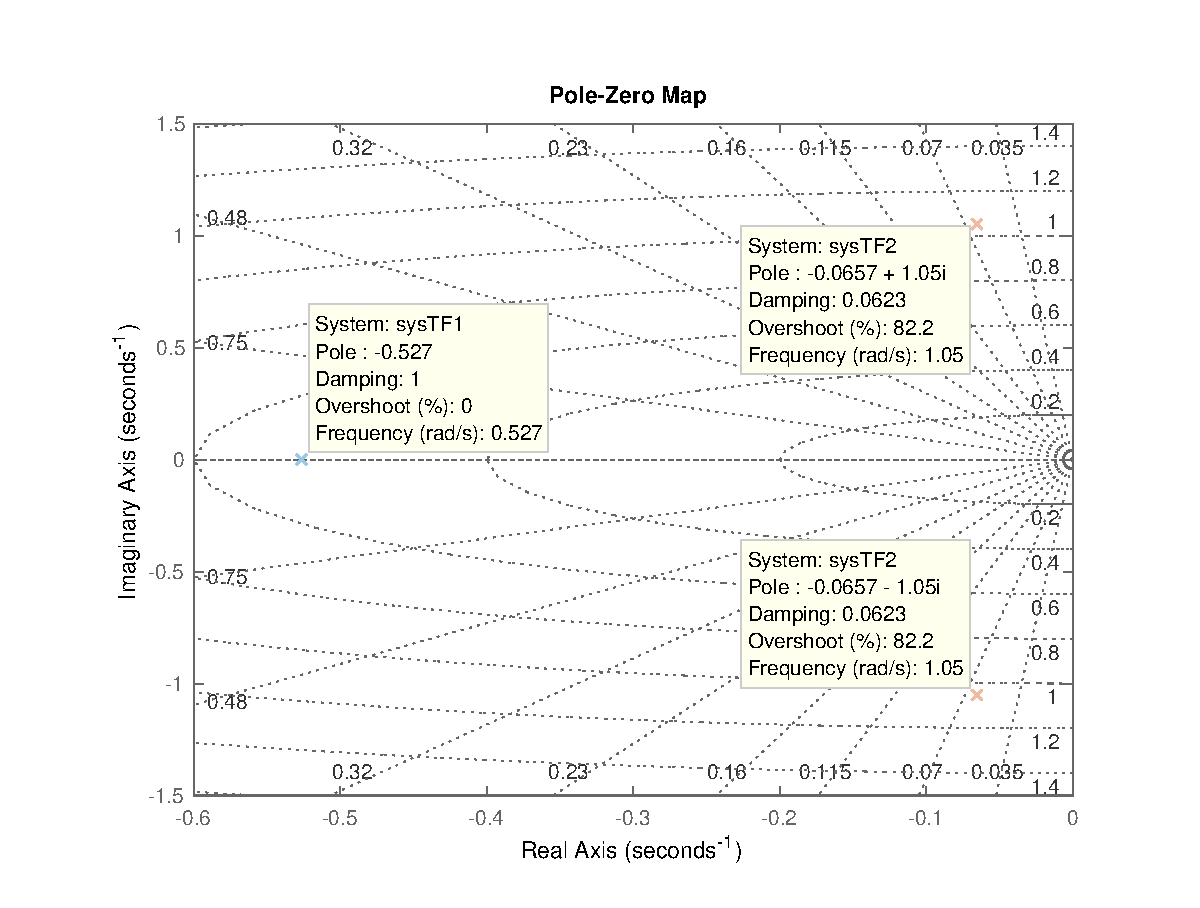
\includegraphics[trim = 35 14 35 0, clip, width=0.55\textwidth]{poleszmap.eps}
  \end{center}
  \caption{Map of the Poles, sysTF1 = First Order, sysTF2 = Second Order}
 \label{poleszmap}
  \vspace{-20pt}
\end{wrapfigure}

Observing Figure \ref{2ndTFcomp} and \ref{1stTFcomp} many deviation's
from MATLAB's theoretical transfer function step response were observed.
During the Quanser operation, a significant observable error was the
drift in the Quanser, more noticeable during longer runs; potentially
due to accumulating error increasing with time. Whilst the Quansers have
error correcting features (through the closed-loop nature of the other
parameters), this is only sensitive to a finite degree so could be
considered imperfect. An initial elevator input was set to -2 (to get
the fans running), and then after 40 seconds an elevator step was input
into the system. As a result the step input may have been applied during
mid oscillation past the steady state elevation position; this likely
either amplified or decreased the actual step input depending on which
stage of oscillation the Quanser was at. A 40 seconds run reduced the
steady-state level to 10-20\% of the steady state value. Errors may
accumulate for a greater run time as the system fails to accurately
correct for inconsistencies.

Another source of deviation is inaccuracy in step input time. In theory
the step input is modelled as an immediate action. A step block was
introduced in the Simulink model to automate the `elevator input' at 40
seconds, however closer observation of the corresponding pitch and
travel data plots revealed a slight delay. Accumulated lag in the system
and controller and a delayed response time both contributed to latency.
Latency causes a phase and amplitude shift in experimental results, as
well as introducing error in parameters such as the logarithmic
decrement \(\Lambda_i\) and damped frequency \(\omega_d\) calculations.

From a mechanical perspective, friction in the Quanser hinge support and
tension from the power cables resulted in a reduction in expected
elevation. This adds to the natural damping of the system, one
explaining for the compacted peaks in experimental data (see Figure
\ref{2ndTFcomp}), and could explain some variation in repeats which was
larger than would be expected for a fixed experiment.

As with any control system, noise can be introduced by external and
internal factors. In the Quanser system, gyro noise and wind resistance
are contributing factors. Sensors in any system measure quantities which
need to be controlled - in this case the elevator sensor sampling was
storing values at discrete points. Whilst the sampling time was quite
small, capturing the general nature of the oscillating damped curves,
some critical points may have been missed. An example can be observed at
the point of highest amplitude, the inflexion behaviour begins after a
region of constant amplitude. Computationally we see a quicker inflexion
transition in this region.

\newpage
